\chapter{Introduction}
\label{chap:introduction}

% Superconductivity has been known for a long time but we don't have an explanation.
% In BCS theory the lattice plays a fundamental role.
% First it seemed that in High-Tc the lattice was not that important.
% Electronic models have been largely unsuccessful so far.
% Several experimental observations (lattice and electronic inhomogeneities, phonon spectra and isotopic effects) suggest that lattice plays a fundamental role, altough in a somewhat different fashion than BCS.
% Electron-lattice correlations could be essential. Maybe in the form of polarons.
% Such correlations can't be adressed with the usual (anti-)adiabatic approximations, so an exact treatment is necessary.
% Exact treatments are computationally expensive so we need to narrow our scope.
% There is evidence of polaronic behaviour in YBCO's O(4)-Cu(1)-O(4).
% A Peierls-Hubbard model has been used there to explain the lattice distortion.
% We explore many other excitations in that model trying to reconcile its predictions with the experimental observations.
% Particular emphasis is given to the isotopic effects because there is controversy around them and they probe the electron-lattice relationship.


\section{Experimental observations}

There are a number of effects related to structural changes in the chain plane of the oxygen-deficient YBa$_{2}$Cu$_{3}$O$_{7-\delta}$ superconductor. 

From \cite{Bahrs2004}

\begin{quote}
Samples quenched from high to about room temperature show spontaneous reordering of oxygen atoms in the chain sites on a time scale between hours and days. 
The structural development has been monitored with x-ray and neutron scattering, both verifying a shortening of the crystallographic axes and the formation of superstructure patterns with full and empty chains for values of oxygen deficiency around $\delta \sim  0.5$. 
[...] the critical temperature of the samples was observed to increase, pointing to the close connection between chain length and carrier concentration in the superconducting planes. 
Calculations of the Cu1 valence in different oxygen surroundings explain the charge transfer involved. 
This correlation between structure and electrical properties has also been shown by application of pressure, after which the critical temperature also remains enhanced as long as the sample is kept cool, but relaxes when it is warmed up to room temperature. 
Other metastable effects are induced by illumination, such as persistent photoconductivity, where after exposure to visible light conductivity and, in superconducting samples, critical temperature show a metastable increase.
\end{quote}

\subsection{Structural inhomogeneity}

See introduction of this article: \cite{Ivanov1995}

The parent compounds of cuprate superconductors form ordered crystalline structures and exhibit antiferromagnetic order at low temperatures. 
However,  in compounds like La$_{1.85}$Sr$_{0.15}$CuO$_{4}$ and La$_{2}$CuO$_{4.1}$, the dopant atoms necessary to achieve a superconducting compound are not placed at the crystal symmetry allowed sites yielding to intrinsically structurally inhomogeneous systems\cite{Poccia2011}. 
While in other cases, like YBCO$_{6+\delta}$, extra dopant atoms reside in crystal symmetric positions but the departure from stoichiometry yields compositional disorder\cite{Chen1988} \cite{Andersen1990} with the same consequence. 
In these systems the crystalline translational symmetry is broken. 
Although from the structural inhomogeneity does not necessarily follow an inhomogeneous electronic ground state, for some regions of the phase diagram, depending on the dopant concentration, such state is realized. 
This region of phase space has been identified as the pseudogap phase\cite{Kresin2009} \cite{Muller2007} \cite{Timusk1999}. 
An important consideration is that, although the dopant atoms are at fixed positions, the structural inhomogeneity has a dynamical character\cite{Mihailovic2005} \cite{Bianconi1996} and is present even in compounds with perfect crystallographic symmetry like HoBa$_{2}$Cu$_{4}$O$_{8}$\cite{RubioTemprano2000}. 
In addition to the breaking of the crystalline translational symmetry the pseudogap phase exhibits other broken symmetries. 
Time-reversal symmetry breaking was found using angular resolved photoemission spectroscopy with circularly polarized photons in Bi$_{2}$Sr$_{2}$CaCu$_{2}$O$_{8+\delta}$\cite{Kaminski2002}. 
It was also found, by x-ray absorption spectroscopy, that the crystalline rotational symmetry is broken locally in La$_{1.85}$Sr$_{0.15}$CuO$_{4}$ with alternating regions of tetragonal and orthorhombic symmetry \cite{Bianconi1996}. 
A perspective of the observation of broken symmetries in high-T$_{c}$ superconductors, emphasizing that some of these broken symmetries are hidden from common observational techniques, is discussed in ref.\cite{Chakravarty2011}. The clues provided by these broken symmetries should yield an understanding of the ground state in this pseudogap phase, its elementary excitations and the appearance of superconductivity at temperatures below the onset of the pseudogap. 

\subsection{Dynamical local lattice distortions}

Local lattice distortion were reported in a two-site distribution for the Cu(1)-apical oxygen in YBa$_{2}$Cu$_{3}$O$_{7}$  at temperatures above T$_{c}$ using Cu K-edge EXAFS \cite{MustredeLeon1990, Conradson1990}. 
This results were controversial\cite{Kwei1990} since they seemed to contadict diffraction experiments (which have a precision of ~0.001Å\cite{Miceli1988}. 
However the EXAFS results showed two sites separated by ~0.11Å that changed into a single site distribution near the superconducting transition temperature.

\begin{figure}[ht!]
\centering
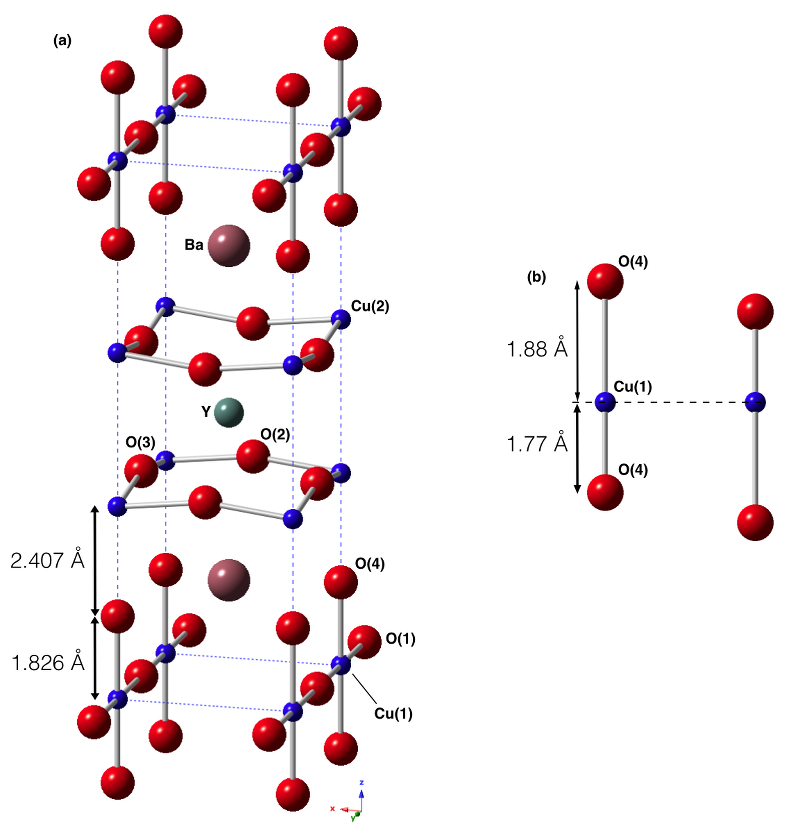
\includegraphics[width=0.8\textwidth]{images/YBCO_O-Cu-Ov2.jpg}
\caption{\textbf{(a)} Crystal structure of YBa$_{2}$Cu$_{3}$O$_{7}$. The dashed line denotes de unit cell. \textbf{(b)} The two possible configurations in the O(4)-Cu(1)-O(4) cluster due to the split O-Cu bond distances (not to scale).
}
\label{fig:YBCO_structure}
\end{figure}


\subsection{Electronic inhomogeneity}
\subsection{Phonon spectra}
\subsection{Isotopic effects}

It is possible to make a site-selective substitution $^{16}$O $\rightarrow$ $^{18}$O in YBCO \cite{Conder1993} allowing a precise study of the isotopic effects. 
This has effects in both the phonon frequencies \cite{Ruani1994} and T$_{c}$ \cite{Zech1994,Cardona1988}. 
The \textit{harmonic} approximation accounts well for the O(2)/O(3) vibrations but it fails for O(4) (see again \cite{Ruani1994})

Noticeable isotopic shifts have been used to identify particular excitations as \textit{phononic} in origin (v.g. \cite{Thomsen1990}) however, we will argue, the converse is not true. 
That is, there can be \textit{phononic} excitations without a measurable isotopic shift.

